\chapter{AI Component Design}
\label{chap:ai-component-design}

% \section{Software Development Methodology}
% \label{section:software-development-methodology}
% <TIP: Describe your software development methodology in this section. />

% \section{Technology Stack}
% \label{section:technology-stack}
% <TIP: Describe your technology stack here. See the following example from ThaiProgrammer.org />
% \begin{figure}[h]
%     \centering
%     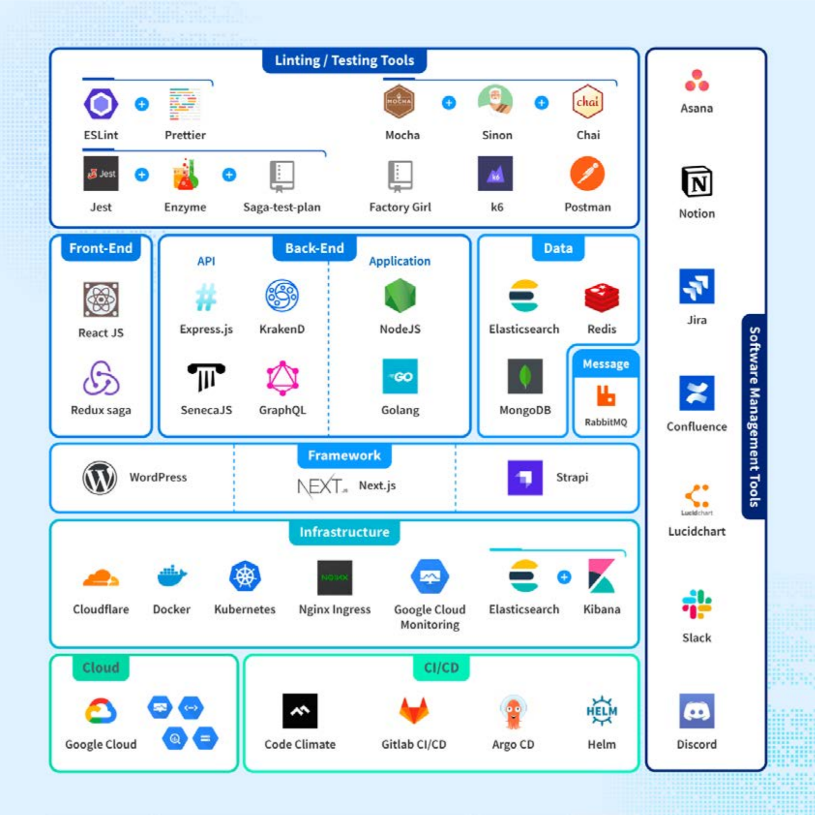
\includegraphics[width=0.5\textwidth]{examples/tech-stack.png}
%     \caption{Example technology stack}
% \end{figure}

% \section{Coding Standards}
% \label{section:coding-standards}
% <TIP: Describe your coding standard for this project here. />

% \section{Progress Tracking Report}
% \label{section:progress-tracking-report}
% <TIP: Show that you have been working on this project overtime.
% It can be in the form of a burndown chart or a contribution graph from GitHub./>

\section{Business Context \& AI Integration}
\label{section:business-context-ai-integration}

KU Parking has integrated model for the detection of available parking spots. Figure \ref{fig:overview-system-flow} provides a system overview: surveillance cameras monitor the parking area, feeding video to a local surveillance footage server. Periodically, individual frames from the video stream are extracted and processed by the model (as outlined in Figure \ref{fig:model-flow}). The model performs object detection to locate both cars and parking spaces within the image. Subsequently, it calculates the Intersection over Union (IoU), a metric quantifying the overlap between each detected vehicle's bounding box and the defined area of a parking spot. By comparing the IoU against a set threshold, the system determines if a vehicle significantly occupies a parking space, thus indicating its availability. This output is served to the client by the service server.

By integrating a detection model, KU Parking can reduce the cost of installing a parking indication system by leveraging existing infrastructure. To inform users, parking availability requires continuous monitoring, as the availability and usage of parking spots can change throughout the day. The model helps automate this continuous monitoring process by analyzing feeds, providing up-to-date information on parking spot occupancy. The incorrect detections typically result in minor user frustration rather than significant damage.

\begin{figure}[H]
    \centering
    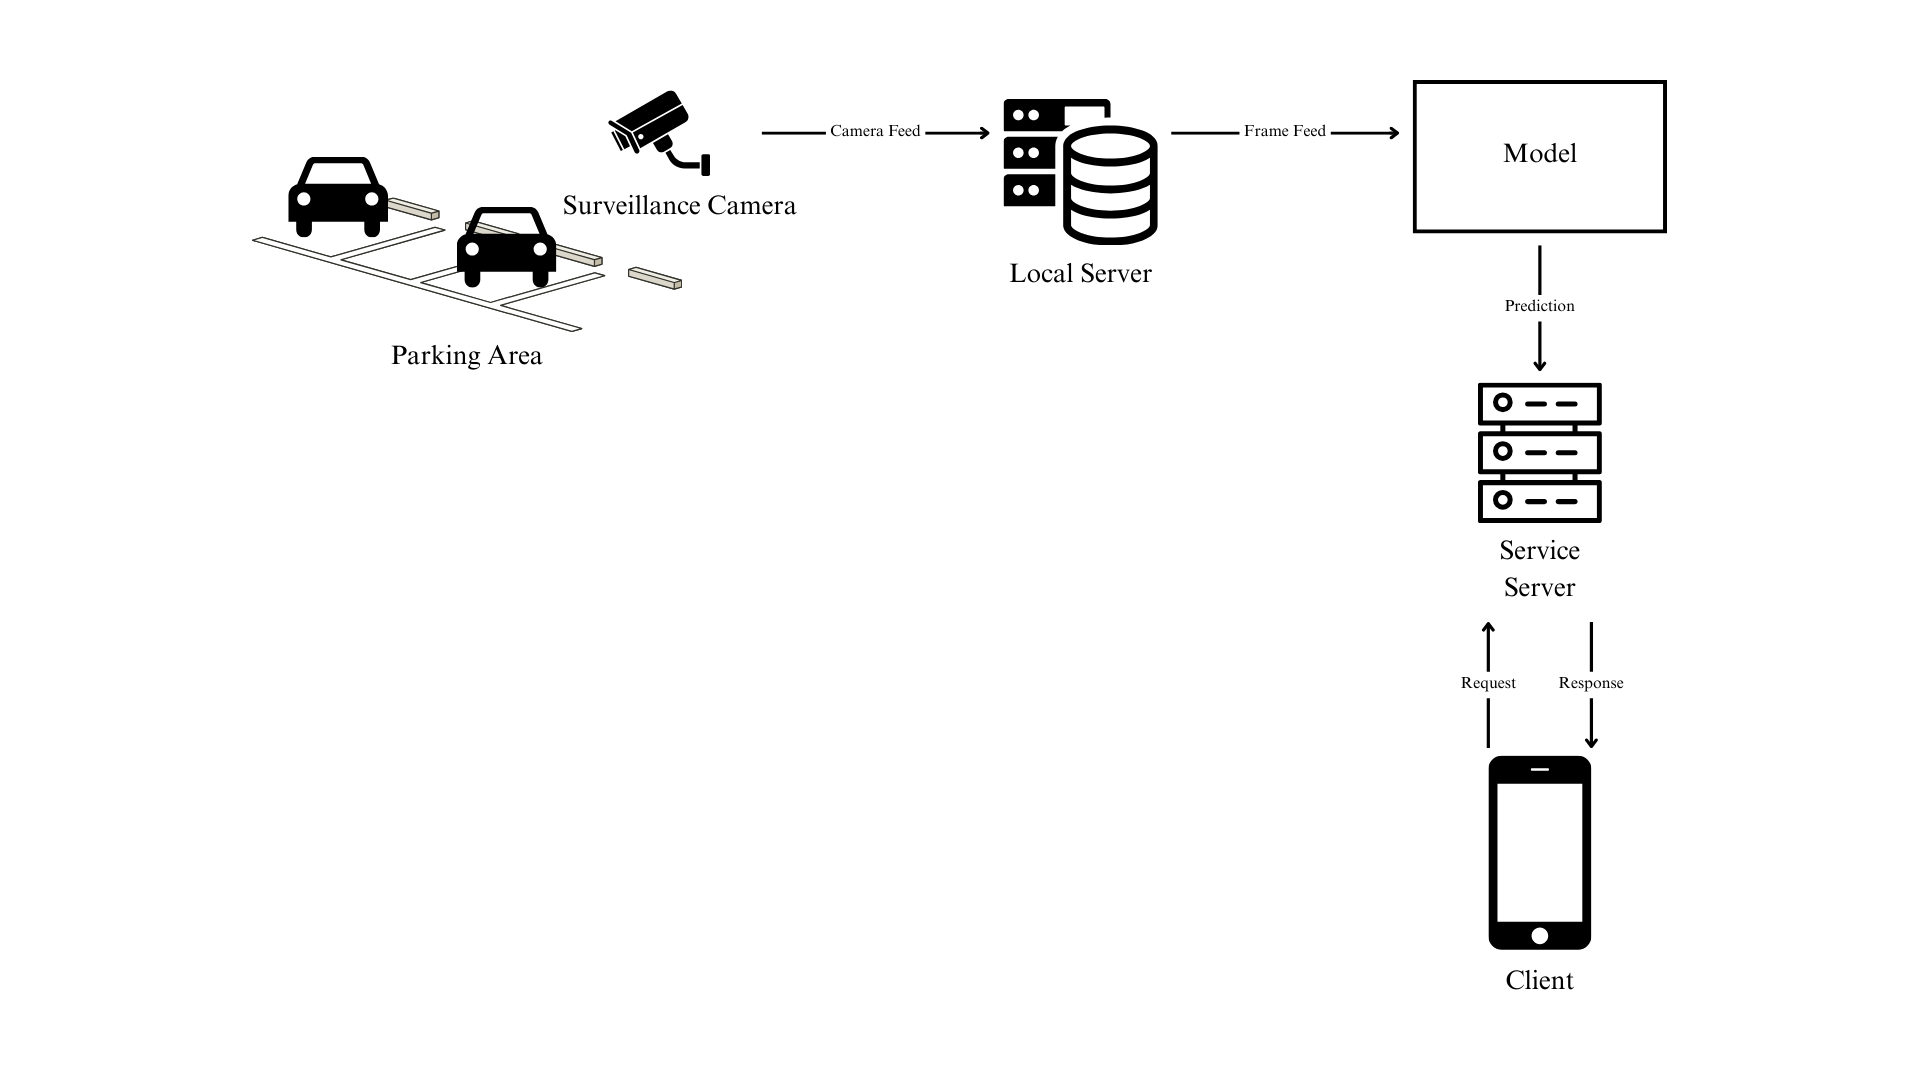
\includegraphics[width=\textwidth,keepaspectratio]{diagrams/system-flow/overview-system-flow.png}
    \caption{Overview System Flow}
    \label{fig:overview-system-flow}
\end{figure}

\begin{figure}[H]
    \centering
    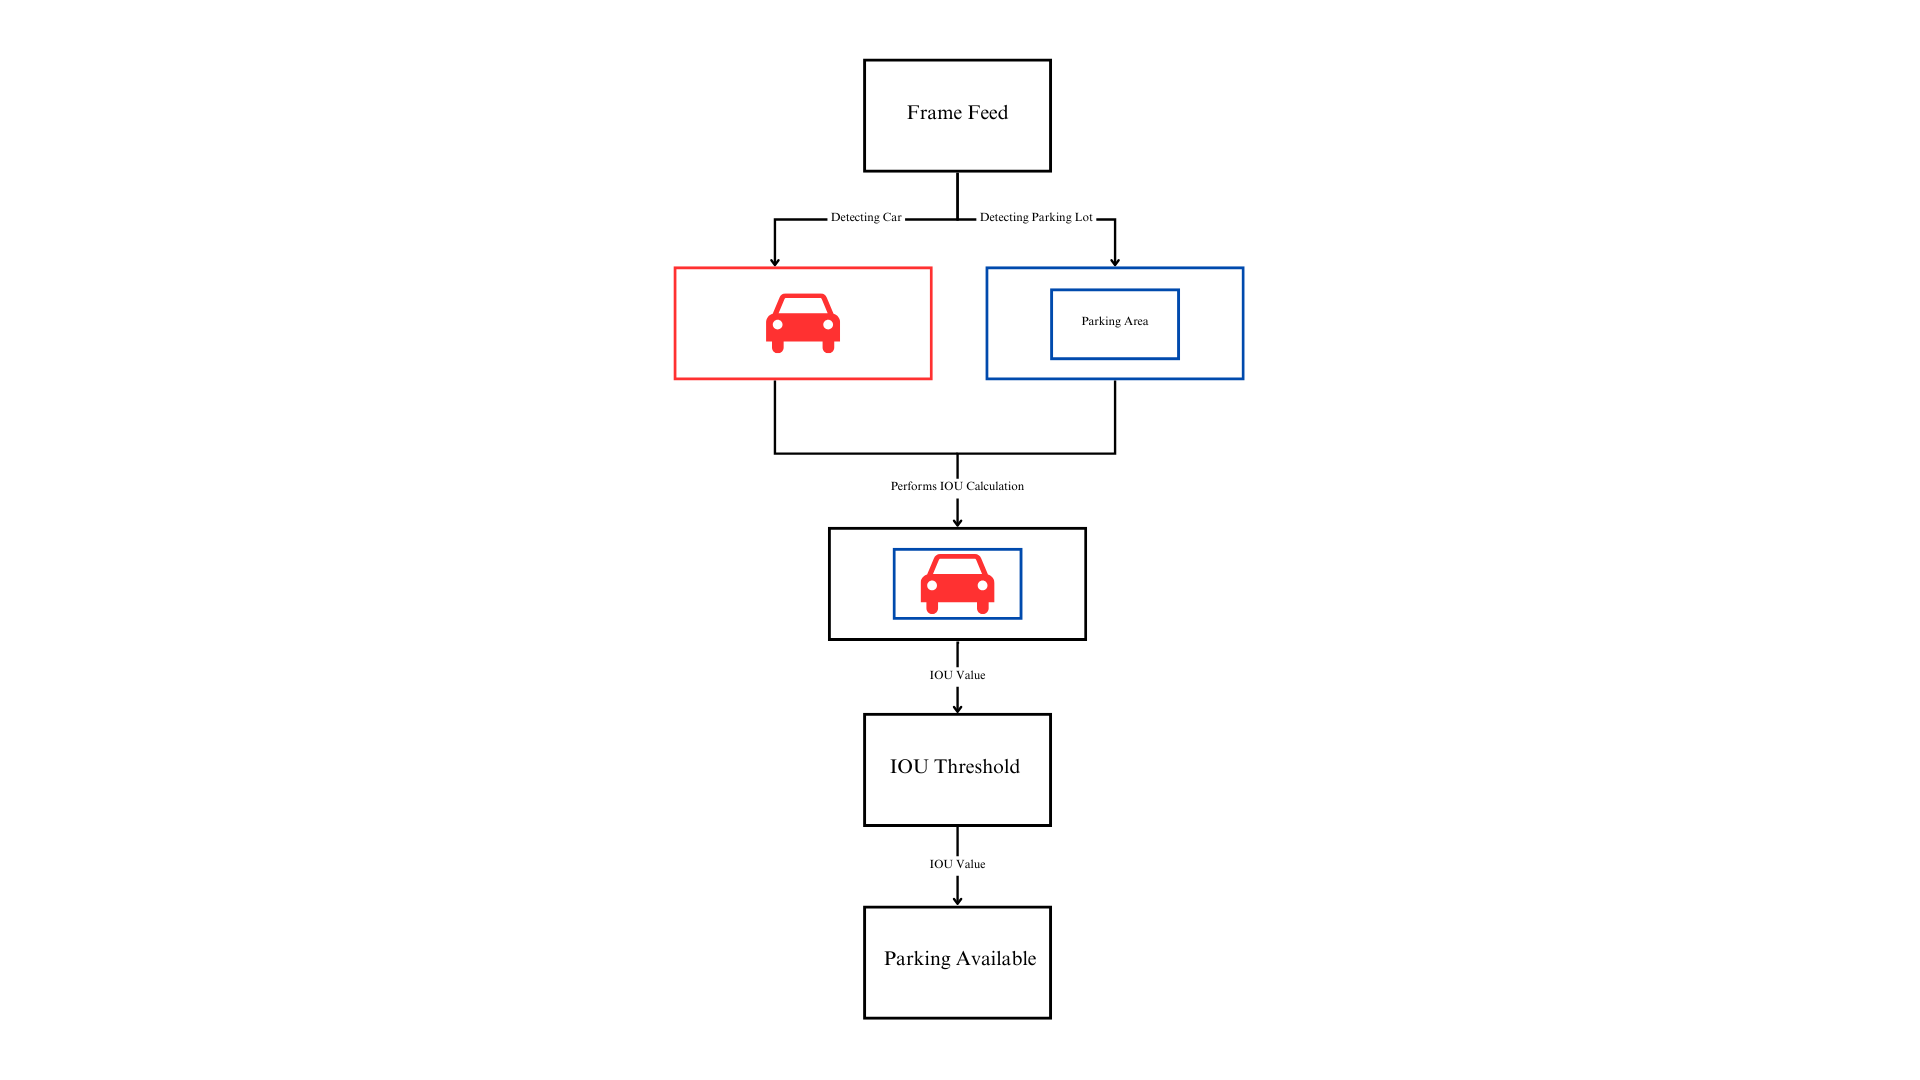
\includegraphics[width=\textwidth,keepaspectratio]{diagrams/system-flow/model-flow.png}
    \caption{Detection Model Flow}
    \label{fig:model-flow}
\end{figure}

\clearpage
\section{Goal Hierarchy}
\label{section:goal-hierarchy}

The tables in this section outline the goals for the KU Parking system at different levels: Organizational (Table \ref{tab:organization-goal}), System (Table \ref{tab:system-goal}), User (Table \ref{tab:user-goal}), and AI Model (Table \ref{tab:ai-model-goal}). Each table details the goal, how it will be measured, the data collection, and the operationalization.

\begin{table}[H]\caption{Organizational Goals of KU Parking}
    \label{tab:organization-goal}
    \centering
    \resizebox{\textwidth}{!}{ 
        \begin{tabular}{|p{4cm}|p{4cm}|p{4cm}|p{4cm}|} 
            \hline
            \textbf{Organizational Goals} & \textbf{Identified Measure} & \textbf{Data Collection} & \textbf{Operationalization} \\
            \hline
            Enhance on-campus driver experience & User satisfaction rating & User feedback survey, app usage analytics & Regular user satisfaction surveys and Usage frequency \\
            \hline
            Promote campus development with cost-effective technology & System installation and maintenance cost and alternatives & Record of KU Parking development and deployment expenses & Compare installation and operational costs to alternatives \\
            \hline
        \end{tabular}
    }
\end{table}

\begin{table}[H]\caption{System Goals of KU Parking}
    \label{tab:system-goal}
    \centering
    \resizebox{\textwidth}{!}{ 
        \begin{tabular}{|p{4cm}|p{4cm}|p{4cm}|p{4cm}|} 
            \hline
            \textbf{System Goals} & \textbf{Identified Measure} & \textbf{Data Collection} & \textbf{Operationalization} \\
            \hline
            Provide availability of the parking spots & Detection accuracy, latency & Model output compare to real status & Percentage of correct indication \\
            \hline
            Presenting alternative parking area & Number of parking between parking area & Logs of number of parking car around the same area & Compare parking data between parking areas within the close area \\
            \hline
        \end{tabular}
    }
\end{table}

\begin{table}[H]\caption{User Goals of KU Parking}
    \label{tab:user-goal}
    \centering
    \resizebox{\textwidth}{!}{ 
        \begin{tabular}{|p{4cm}|p{4cm}|p{4cm}|p{4cm}|} 
            \hline
            \textbf{User Goals} & \textbf{Identified Measure} & \textbf{Data Collection} & \textbf{Operationalization} \\
            \hline
            Quickly find optimal available parking spaces & User satisfaction rating & User feedback survey, app usage analytics & Regular user satisfaction surveys and Usage frequency \\
            \hline
        \end{tabular}
    }
\end{table}

\begin{table}[H]\caption{AI Model Goals of KU Parking}
    \label{tab:ai-model-goal}
    \centering
    \resizebox{\textwidth}{!}{ 
        \begin{tabular}{|p{4cm}|p{4cm}|p{4cm}|p{4cm}|} 
            \hline
            \textbf{AI Model Goals} & \textbf{Identified Measure} & \textbf{Data Collection} & \textbf{Operationalization} \\
            \hline
            Accurately detect vacant space & Precision, recall, F1 score & Annotated images, prediction logs & Model evaluation using labeled datasets \\
            \hline
            Operate efficiently in close to real time & Latency & System logs & Measure average time used for processing per image/frame \\
            \hline
        \end{tabular}
    }
\end{table}

\clearpage
\section{Task Requirements Analysis Using AI Canvas}
\label{section:task-requirement-analysis-using-ai-canvas}
\subsection{AI Task Requirements}
\label{subsection:ai-task-requirement}
\begin{itemize}
  \item \textbf{Requirements (REQ)}
  \begin{itemize}
    \item Detect the occupancy status of each parking spot using frames from video feeds from existing surveillance cameras.
    \item Operate with high precision and recall to minimize false positives and negatives in vehicle detection.
    \item Continuously monitor multiple parking areas to reflect up-to-date status across campus.
  \end{itemize}
  \item \textbf{Specifications (SPEC)}
  \begin{itemize}
    \item Use the YOLO (You Only Look Once) object detection model to identify vehicles in each video frame.
    \item Define parking spot boundaries through edge detection assistance and manual annotation during initial setup.
    \item Apply the Intersection over Union (IoU) algorithm to compare vehicle bounding boxes with parking space boundaries. If the IoU exceeds a predefined threshold, the system marks the space as occupied; otherwise, it is marked as vacant.
  \end{itemize}
  \item \textbf{Environment (ENV)}
  \begin{itemize}
    \item Operates on surveillance camera feeds installed around campus.
    \item Handles variable frame quality and angles depending on the camera position.
    \item Integrated into a cloud-based system for centralized processing and data delivery to a mobile application.
    \item Operates in near real-time, ensuring timely updates to parking availability status.
  \end{itemize}
\end{itemize}


\subsection{AI Canvas Development}
\label{subsection:ai-canvas-development}
The KU Parking Machine Learning Canvas (Table \ref{tab:ml-canvas}) outlines how AI component in KU Parking was designed and evaluated.

\begin{table}[H]
\centering
\caption{KU Parking Machine Learning Canvas}
\label{tab:ml-canvas}
\begin{tabular}{|p{4cm}|p{10cm}|}
\hline
\multicolumn{2}{|c|}{\cellcolor{cyan!15}\textbf{PREDICT}} \\ \hline
\textbf{Decisions} & Determine whether each parking space is occupied or vacant.\\ \hline
\textbf{ML Task} & Car Detection (YOLO) on surveillance frames and postprocessing (IoU) to determine parking spot status.\\ \hline
\textbf{Making Predictions} & Run on set interval and frequency\\ \hline
\textbf{Offline Evaluation} & Use precision, recall, and F1-score on validation data. \\ \hline

\multicolumn{2}{|c|}{\cellcolor{yellow!15}\textbf{LEARN}} \\ \hline
\textbf{Data Sources} & Video frames from campus surveillance cameras and other surveillance footage (for training). \\ \hline
\textbf{Collecting Data} & Frames are periodically extracted and labeled (for parking spot boundaries). \\ \hline
\textbf{Features} & Bounding boxes of vehicles from YOLO and parking boundaries annotated manually with edge detection assist. \\ \hline
\textbf{Building Models} & Train YOLO-based model with annotated images. Use IoU threshold to determine parking status. \\ \hline

\multicolumn{2}{|c|}{\textbf{GOAL}} \\ \hline\textbf{Value Propositions} & Reduce installation cost for campus and improve parking efficiency with parking availability detection model. \\ \hline

\multicolumn{2}{|c|}{\cellcolor{purple!15}\textbf{EVALUATE}} \\ \hline
\textbf{Live Evaluation and Monitoring} & Monitor prediction latency and matrices from periodically collected frames. Compare predictions with actual usage data and feedback. \\ \hline

\end{tabular}
\end{table}

\clearpage
\section{User Experience Design with AI}
\label{section:user-experience-with-ai}
The AI component of KU Parking is designed to detect and identify the availability of parking spaces. Users receive information based on the results of the detection model, as illustrated in the User Interface Design section (Section \ref{section:user-interface-design}).

Additionally, users can provide feedback in cases of incorrect parking availability detection by submitting a report through the parking information interface, as shown in Figure \ref{fig:ui_parking_information}.

The detection model plays a key role in identifying the availability of parking spaces in real time. By analyzing input from surveillance cameras, the model can determine whether a parking spot is occupied or vacant. This approach significantly reduces the need for installing parking indication systems, such as sensor-based indicators, or relying on manual monitoring by personnel. As outlined in the system's benefits, this approach helps lowers installation and maintenance costs.

\begin{figure}[h]
    \centering
    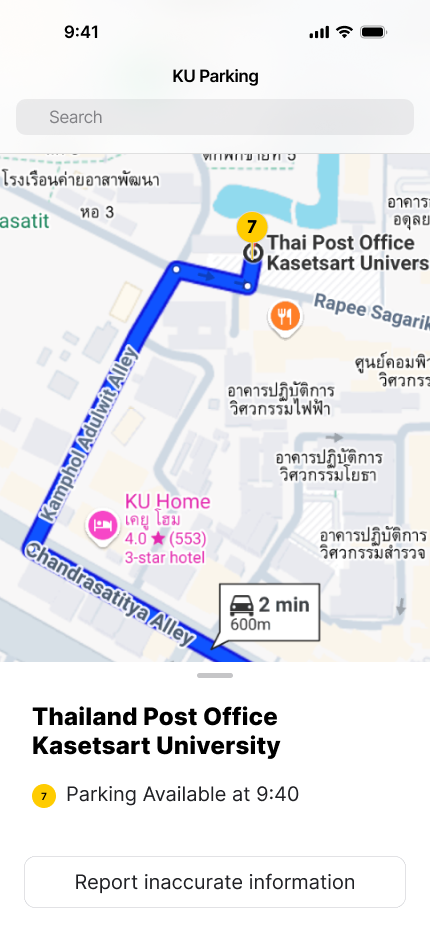
\includegraphics[width=0.5\textwidth]{ui-design/parking-information.png}
    \caption{User Interface Design for Parking information}
    \label{fig:ui_parking_information}
\end{figure}
